\chapter{Visualisation implementation}\label{C:sd}
This chapter discusses the implementation of the visulisation uisng the designs discussed previously. It details the tools used, the deliverables produced, and the problems encountered
%It details decisions made during the project such as choosing a viable framework, the choice of extending a previous system, platform choice, and designs of the actual system.   
\section{Tools and artifacts used}



\subsection{Main system}
In addition to Processing in the main system there was an additional opensource library required for effective user interface components, this library was called
\begin{itemize}
 \item ControlP5 REF~
\end{itemize}


\subsection{Kinect sensor system}
The Microsoft Kinect sensor required 3 additional libraries to integrate with Processing, these were:
\begin{enumerate}
 \item NITE ref~
 \item SimpleOpenNi ref~
\end{enumerate}
These libraries provided drivers to run the Kinect sensor in Processing as well as basic gesture recognition and body tracking. However as the libraries were opensource due to the official Kinect SDK not being compatible with Processing, the gesture recognition was not as user friendy or effective as the official libraries. The effect of this was that the gesture tracking used in the system had to be .... ~
\section{Implementation of planned features}
All of the features that were planned were completed for the visualisation, this is including the additional work that was planned around the Kinect sensor.

Below is a description of each of the main visualisation features that were completed.
Image of navigation window

\begin{figure}[h!]
  \centering
      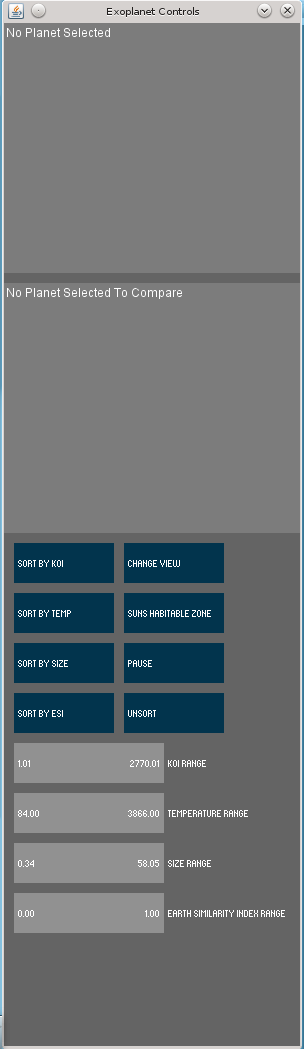
\includegraphics[width=0.3\textwidth]{images/nav.png}
  \caption{Navigation Panel Overview}
  \label{fig:nav}
\end{figure}


\begin{figure}[h!]
  \centering
      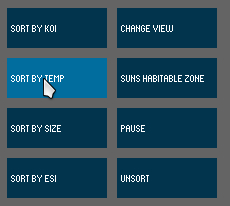
\includegraphics[width=0.6\textwidth]{images/buttons.jpg}
  \caption{Panel of interactive buttons}
  \label{fig:buttons}
\end{figure}

Image of each slider
\begin{figure}[h!]
  \centering
      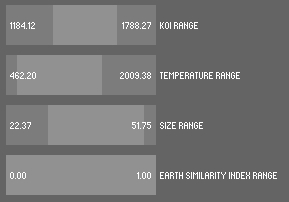
\includegraphics[width=0.6\textwidth]{images/sliders.jpg}
  \caption{Panel of interactive range sliders}
  \label{fig:sliders}
\end{figure}
Image of text boxes

Image of using kinect system

Image of using non kinect system

\section{Problems encountered}
Due to the number of elements that needed to be displayed on screen at any one time (ie 2234 exoplanets), the load placed on a system is very high due to the need to render 2234 eclipses to represent the planets. This uncovered a bug in the processing library in which the memory use of the visualisation would periodically increase until it crashed due to an out of memory exception. After much experimentation of how to overcome this issue, I discovered that rather than trying to render a native elipse shape in processing, if I instead rendered a Scalable Vector Graphic this bug would not manifest. 
\\\\
Libraries used for gesture detection in kinect are opensource in order to work with processing did not have decent detection
\\\\
Using the Processing framework meant using a non industrial???~ IDE that had many bugs, for example when undoing multiple times in a row the file being modified would periodically become corrupted by lines of code being taken away or inserted into the wrong locations. The solution to this issue was to ensure that I regularily commited any changes to my version controlled system on Github ((REFERBTECE ~)). Doing this meant that if at any time a file became corrupted I could easily see the changes in the file when compared against the precious commit and manually fix the file. 
\\\\
Performance limitations
SCREENSHOT ~